\documentclass{article}
\usepackage{graphicx}
\usepackage{IEEEtrantools}
\usepackage{amsmath}

\title{Solve $Z_1 = Z_2$ for $x_1$}
\author{Daniel Fishbein}

\begin{document}
\maketitle

\section{Given:}

\begin{figure}[h!]{
    \centering
    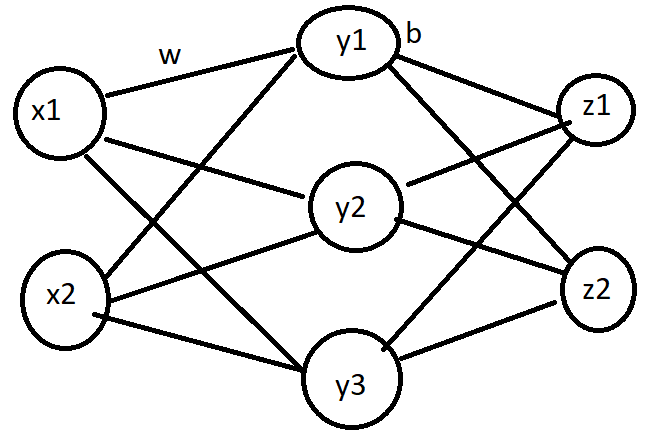
\includegraphics[width=0.5\linewidth]{Given_NN.png}
    \caption{Given Neural Net}\label{fig:NeuralNet}
    }
\end{figure}

\hbox{Figure~\ref{fig:NeuralNet} shows the given Neural Net that will be analysed.}

\vspace{5mm}
\hbox{$x_1, x_2$ are the input neurons}
\hbox{$y_1, y_2, y_3$ are the hidden layers neurons}
\hbox{$z_1, z_2$ are the output neurons}

\vspace{2mm}
\hbox{$w$ denotes a weight}
\hbox{$w_{y_1->z_2}$ denotes the weight from $y_1$ to $z_2$}

\vspace{2mm}
\hbox{$b$ deontes a bias}
\hbox{$b_{y_3}$ deontes the bias associated with neuron $y_3$}

\vspace{5mm}
\hbox{The input to a $y_i$ neuron will be denoted as:}
\hbox{$y_i = \sigma(w_{x_1->y_i} * x_1 + w_{x_2->y_i} * x_2 + b_{y_i} )$}

\vspace{2mm}
\hbox{Where $\sigma(x) = \frac{1}{1+e^{-x}} = \frac{1}{1+\exp[-x]}$}

\vspace{5mm}
\hbox{The input to a $z_i$ neuron will be denoted as:}
\hbox{$z_i = \sigma(w_{y_1->z_i}*y_1 + w_{y_2->z_i}*y_2 + w_{y_3->z_i}*y_3 + b_{z_i} )$}




\section{Solve $z_1 = z_2$ for $x_1$}
\begin{equation}
    z_1 = z_2    
\end{equation}

\begin{equation}
    z_1 = \sigma(
        w_{y_1->z_1}*y_1 + 
        w_{y_2->z_1}*y_2 + 
        w_{y_3->z_1}*y_3 + b_{z_1})   
\end{equation}


\begin{multline}
        z_1 = \sigma(
            w_{y_1->z_1}*\sigma(
                    w_{x_1->y_1} * x_1 + 
                    w_{x_2->y_1} * x_2 + b_{y_1})\\
            + w_{y_2->z_1}*\sigma(
                    w_{x_1->y_2} * x_1 + 
                    w_{x_2->y_2} * x_2 + b_{y_2})\\ 
            + w_{y_3->z_1}*\sigma(
                    w_{x_1->y_3} * x_1 + 
                    w_{x_2->y_3} * x_2 + b_{y_3})\\
            + b_{z_1})
\end{multline}

\begin{multline}
    z_2 = \sigma(
        w_{y_1->z_2}*\sigma(
                w_{x_1->y_1} * x_1 + 
                w_{x_2->y_1} * x_2 + b_{y_1}) \\
        + w_{y_2->z_2}*\sigma(
                w_{x_1->y_2} * x_1 + 
                w_{x_2->y_2} * x_2 + b_{y_2})\\ 
        + w_{y_3->z_2}*\sigma(
                w_{x_1->y_3} * x_1 + 
                w_{x_2->y_3} * x_2 + b_{y_3})\\
        + b_{z_2})
\end{multline}

\begin{multline}
    (1+\exp[- (w_{y_1->z_1}* \frac{1}{1+\exp[
            w_{x_1->y_1} * x_1 + 
            w_{x_2->y_1} * x_2 + b_{y_1}]}\\
        + w_{y_2->z_1}* \frac{1}{1+\exp[
            w_{x_1->y_2} * x_1 + 
            w_{x_2->y_2} * x_2 + b_{y_2}]}\\
        + w_{y_3->z_1}* \frac{1}{1+\exp[
            w_{x_1->y_3} * x_1 + 
            w_{x_2->y_3} * x_2 + b_{y_3}]}\\
    + b_{z_1})])^{-1}
    \\=\\
    (1+\exp[- (w_{y_1->z_2}* \frac{1}{1+\exp[   
            w_{x_1->y_1} * x_1 + 
            w_{x_2->y_1} * x_2 + b_{y_1}]}\\
        + w_{y_2->z_2}*\frac{1}{1+\exp[
            w_{x_1->y_2} * x_1 + 
            w_{x_2->y_2} * x_2 + b_{y_2}]}\\
        + w_{y_3->z_2}*\frac{1}{1+\exp[
            w_{x_1->y_3} * x_1 + 
            w_{x_2->y_3} * x_2 + b_{y_3}]}\\
    + b_{z_2})])^{-1}\\
\end{multline}

\hbox{NOTE\@: this equation is too big. Lets scope it down.}
\hbox{Define:}
\begin{IEEEeqnarray}{rCl}
    B_1 = -w_{x_1->y_1} * x_1 + w_{x_2->y_1} * x_2 + b_{y_1}\\
    B_2 = -w_{x_1->y_2} * x_1 + w_{x_2->y_2} * x_2 + b_{y_2}\\
    B_3 = -w_{x_1->y_3} * x_1 + w_{x_2->y_3} * x_2 + b_{y_3}\\
\end{IEEEeqnarray}

\hbox{NOTE\@: Substatuting B in.}

\begin{IEEEeqnarray}{rCl}
    (1+\exp[- (w_{y_1->z_1}* \frac{1}{1+\exp[B_1]}\\
        + w_{y_2->z_1}* \frac{1}{1+\exp[B_2]}\\
        + w_{y_3->z_1}* \frac{1}{1+\exp[B_3]}\\
        + b_{z_1})])^{-1}
        \\=\\
    (1+\exp[- (w_{y_1->z_2}* \frac{1}{1+\exp[B_1]}\\
        + w_{y_2->z_2}*\frac{1}{1+\exp[B_2]}\\
        + w_{y_3->z_2}*\frac{1}{1+\exp[B_3]}\\
        + b_{z_2})])^{-1}
\end{IEEEeqnarray}


\hbox{Define A}

\begin{IEEEeqnarray}{rCl}
    A_1 = w_{y_1->z_1}* \frac{1}{1+\exp[B_1]}\\
        + w_{y_2->z_1}* \frac{1}{1+\exp[B_2]}\\
        + w_{y_3->z_1}* \frac{1}{1+\exp[B_3]}\\
        + b_{z_1}
\end{IEEEeqnarray}

\begin{IEEEeqnarray}{rCl}
    A_2 = w_{y_1->z_2}* \frac{1}{1+\exp[B_1]}\\
    + w_{y_2->z_2}*\frac{1}{1+\exp[B_2]}\\
    + w_{y_3->z_2}*\frac{1}{1+\exp[B_3]}\\
    + b_{z_2}
\end{IEEEeqnarray}

\newpage
\hbox{NOTE\@: Substatuting A in.}

\begin{equation}
    (1+\exp[- (A_1)])^{-1}
        \\=\\
    (1+\exp[- (A_2)])^{-1}
\end{equation}

\begin{equation}
    (1+\exp[- (A_1)])
        =
    (1+\exp[- (A_2)])
\end{equation}

\begin{equation}
    1+\exp[- (A_1)]
        =
    1+\exp[- (A_2)]
\end{equation}

\begin{equation}
    \exp[- (A_1)]
        =
    \exp[- (A_2)]
\end{equation}

\begin{equation}
    (A_1)
        =
    (A_2)
\end{equation}

\begin{equation}
    A_1
        =
    A_2
\end{equation}

\hbox{Sub in the values of $A_1$ and $A_2$}

\begin{multline}
    \\
        w_{y_1->z_1}* \frac{1}{1+\exp[B_1]}
        + w_{y_2->z_1}* \frac{1}{1+\exp[B_2]}
        + w_{y_3->z_1}* \frac{1}{1+\exp[B_3]}\\
        + b_{z_1}
        \\=\\
        w_{y_1->z_2}* \frac{1}{1+\exp[B_1]}
        + w_{y_2->z_2}*\frac{1}{1+\exp[B_2]}
        + w_{y_3->z_2}*\frac{1}{1+\exp[B_3]}\\
        + b_{z_2}
    \\
\end{multline}


\begin{multline}
    \\
        \frac{w_{y_1->z_1}}{1+\exp[B_1]}
        + \frac{w_{y_2->z_1}}{1+\exp[B_2]}
        + \frac{w_{y_3->z_1}}{1+\exp[B_3]}
        + b_{z_1}
        \\=\\
        \frac{w_{y_1->z_2}}{1+\exp[B_1]}
        + \frac{w_{y_2->z_2}}{1+\exp[B_2]}
        + \frac{w_{y_3->z_2}}{1+\exp[B_3]}
        + b_{z_2}
    \\
\end{multline}

\hbox{Multiply by botoms to create common denominators.}
\begin{multline}
        \\
        \frac{w_{y_1->z_1} * (1+\exp[B_2]) * (1+\exp[B_3])}
            {(1+\exp[B_1]) * (1+\exp[B_2]) * (1+\exp[B_3])} +\\
        \frac{w_{y_2->z_1} * (1+\exp[B_1]) * (1+\exp[B_3])}
            {(1+\exp[B_2]) * (1+\exp[B_1]) * (1+\exp[B_3])} +\\
        \frac{w_{y_3->z_1} * (1+\exp[B_1]) * (1+\exp[B_2])}
            {(1+\exp[B_3]) * (1+\exp[B_1]) * (1+\exp[B_2])} +\\
            b_{z_1}
         \\=\\
        \frac{w_{y_1->z_2} * (1+\exp[B_2]) * (1+\exp[B_3])}
            {(1+\exp[B_1]) * (1+\exp[B_2]) * (1+\exp[B_3])} +\\
        \frac{w_{y_2->z_2} * (1+\exp[B_1]) * (1+\exp[B_3])}
            {(1+\exp[B_2]) * (1+\exp[B_1]) * (1+\exp[B_3])} +\\
        \frac{w_{y_3->z_2} * (1+\exp[B_2]) * (1+\exp[B_1])}
            {(1+\exp[B_3]) * (1+\exp[B_1]) * (1+\exp[B_2])} +\\
            b_{z_2}
        \\
 \end{multline}

 \hbox{REORDRER DENOMINATORS}
 \begin{multline}
    \\
    \frac{w_{y_1->z_1} * (1+\exp[B_2]) * (1+\exp[B_3])}
        {(1+\exp[B_1]) * (1+\exp[B_2]) * (1+\exp[B_3])} +\\
    \frac{w_{y_2->z_1} * (1+\exp[B_1]) * (1+\exp[B_3])}
        {(1+\exp[B_1]) * (1+\exp[B_2]) * (1+\exp[B_3])} +\\
    \frac{w_{y_3->z_1} * (1+\exp[B_1]) * (1+\exp[B_2])}
        {(1+\exp[B_1]) * (1+\exp[B_2]) * (1+\exp[B_3])} +\\
        b_{z_1}
     \\=\\
    \frac{w_{y_1->z_2} * (1+\exp[B_2]) * (1+\exp[B_3])}
        {(1+\exp[B_1]) * (1+\exp[B_2]) * (1+\exp[B_3])} +\\
    \frac{w_{y_2->z_2} * (1+\exp[B_1]) * (1+\exp[B_3])}
        {(1+\exp[B_1]) * (1+\exp[B_2]) * (1+\exp[B_3])} +\\
    \frac{w_{y_3->z_2} * (1+\exp[B_2]) * (1+\exp[B_1])}
        {(1+\exp[B_1]) * (1+\exp[B_2]) * (1+\exp[B_3])} +\\
        b_{z_2}
    \\
\end{multline}

\hbox{MOVE $b_{z_1}$}
\begin{multline}
    \\
    \frac{w_{y_1->z_1} * (1+\exp[B_2]) * (1+\exp[B_3])}
        {(1+\exp[B_1]) * (1+\exp[B_2]) * (1+\exp[B_3])} +\\
    \frac{w_{y_2->z_1} * (1+\exp[B_1]) * (1+\exp[B_3])}
        {(1+\exp[B_1]) * (1+\exp[B_2]) * (1+\exp[B_3])} +\\
    \frac{w_{y_3->z_1} * (1+\exp[B_1]) * (1+\exp[B_2])}
        {(1+\exp[B_1]) * (1+\exp[B_2]) * (1+\exp[B_3])}
    \\=\\
    \frac{w_{y_1->z_2} * (1+\exp[B_2]) * (1+\exp[B_3])}
        {(1+\exp[B_1]) * (1+\exp[B_2]) * (1+\exp[B_3])} +\\
    \frac{w_{y_2->z_2} * (1+\exp[B_1]) * (1+\exp[B_3])}
        {(1+\exp[B_1]) * (1+\exp[B_2]) * (1+\exp[B_3])} +\\
    \frac{w_{y_3->z_2} * (1+\exp[B_2]) * (1+\exp[B_1])}
        {(1+\exp[B_1]) * (1+\exp[B_2]) * (1+\exp[B_3])} +\\
        b_{z_2} - b_{z_1}
    \\
\end{multline}

\hbox{MOVE THE BIG PIECE}
\begin{multline}
    \\
    \frac{w_{y_1->z_1} * (1+\exp[B_2]) * (1+\exp[B_3])}
        {(1+\exp[B_1]) * (1+\exp[B_2]) * (1+\exp[B_3])} +\\
    \frac{w_{y_2->z_1} * (1+\exp[B_1]) * (1+\exp[B_3])}
        {(1+\exp[B_1]) * (1+\exp[B_2]) * (1+\exp[B_3])} +\\
    \frac{w_{y_3->z_1} * (1+\exp[B_1]) * (1+\exp[B_2])}
        {(1+\exp[B_1]) * (1+\exp[B_2]) * (1+\exp[B_3])} -\\
    \frac{w_{y_1->z_2} * (1+\exp[B_2]) * (1+\exp[B_3])}
        {(1+\exp[B_1]) * (1+\exp[B_2]) * (1+\exp[B_3])} -\\
    \frac{w_{y_2->z_2} * (1+\exp[B_1]) * (1+\exp[B_3])}
        {(1+\exp[B_1]) * (1+\exp[B_2]) * (1+\exp[B_3])} -\\
    \frac{w_{y_3->z_2} * (1+\exp[B_2]) * (1+\exp[B_1])}
        {(1+\exp[B_1]) * (1+\exp[B_2]) * (1+\exp[B_3])}
    \\=b_{z_2} - b_{z_1}
    \\
\end{multline}

\hbox{REORDER FOR SIMMILAR TERMS}
\begin{multline}
    \\
    \frac{w_{y_1->z_1} * (1+\exp[B_2]) * (1+\exp[B_3])}
        {(1+\exp[B_1]) * (1+\exp[B_2]) * (1+\exp[B_3])} -
    \frac{w_{y_1->z_2} * (1+\exp[B_2]) * (1+\exp[B_3])}
        {(1+\exp[B_1]) * (1+\exp[B_2]) * (1+\exp[B_3])} + \\
    \frac{w_{y_2->z_1} * (1+\exp[B_1]) * (1+\exp[B_3])}
        {(1+\exp[B_1]) * (1+\exp[B_2]) * (1+\exp[B_3])} -
    \frac{w_{y_2->z_2} * (1+\exp[B_1]) * (1+\exp[B_3])}
        {(1+\exp[B_1]) * (1+\exp[B_2]) * (1+\exp[B_3])} + \\
    \frac{w_{y_3->z_1} * (1+\exp[B_1]) * (1+\exp[B_2])}
        {(1+\exp[B_1]) * (1+\exp[B_2]) * (1+\exp[B_3])} -
    \frac{w_{y_3->z_2} * (1+\exp[B_2]) * (1+\exp[B_1])}
        {(1+\exp[B_1]) * (1+\exp[B_2]) * (1+\exp[B_3])}
    \\=b_{z_2} - b_{z_1}
    \\
\end{multline}

\hbox{COMBINE LIKE TERMS}
\begin{multline}
    \\
    \frac{w_{y_1->z_1} * (1+\exp[B_2]) * (1+\exp[B_3]) - 
        w_{y_1->z_2} * (1+\exp[B_2]) * (1+\exp[B_3])}
        {(1+\exp[B_1]) * (1+\exp[B_2]) * (1+\exp[B_3])} +\\
    \frac{w_{y_2->z_1} * (1+\exp[B_1]) * (1+\exp[B_3]) - 
        w_{y_2->z_2} * (1+\exp[B_1]) * (1+\exp[B_3])}
        {(1+\exp[B_1]) * (1+\exp[B_2]) * (1+\exp[B_3])} +\\
    \frac{w_{y_3->z_1} * (1+\exp[B_1]) * (1+\exp[B_2]) -
        w_{y_3->z_2} * (1+\exp[B_2]) * (1+\exp[B_1])} 
        {(1+\exp[B_1]) * (1+\exp[B_2]) * (1+\exp[B_3])}
    \\=b_{z_2} - b_{z_1}
    \\
\end{multline}

\hbox{fACTOR COMMON NUMERATORS}
\begin{multline}
    \\
    \frac{(w_{y_1->z_1} - w_{y_1->z_2}) * (1+\exp[B_2]) * (1+\exp[B_3])}
        {(1+\exp[B_1]) * (1+\exp[B_2]) * (1+\exp[B_3])} +\\
    \frac{(w_{y_2->z_1} - w_{y_2->z_2}) * (1+\exp[B_1]) * (1+\exp[B_3])}
        {(1+\exp[B_1]) * (1+\exp[B_2]) * (1+\exp[B_3])} +\\
    \frac{(w_{y_3->z_1} - w_{y_3->z_2}) * (1+\exp[B_1]) * (1+\exp[B_2])} 
        {(1+\exp[B_1]) * (1+\exp[B_2]) * (1+\exp[B_3])}
    \\=b_{z_2} - b_{z_1}
    \\
\end{multline}

\hbox{SANITY CHECK}  
\begin{equation}
    aAB - bAB = (a-b)AB
\end{equation}

\hbox{MULTIPLY BY COMMON DENOMINATOR}
\begin{multline}
    \\
    (w_{y_1->z_1} - w_{y_1->z_2}) * (1+\exp[B_2]) * (1+\exp[B_3]) +\\
    (w_{y_2->z_1} - w_{y_2->z_2}) * (1+\exp[B_1]) * (1+\exp[B_3]) +\\
    (w_{y_3->z_1} - w_{y_3->z_2}) * (1+\exp[B_1]) * (1+\exp[B_2]) 
    \\= (b_{z_2} - b_{z_1}) * ((1+\exp[B_1]) * (1+\exp[B_2]) * (1+\exp[B_3]))
    \\
\end{multline}

\hbox{The next step is to multiply this out and emilimate terms. I do not want to do that rn :/}




\newpage
\hbox{GO BACK TO EQ.34}
\begin{multline}
    \\
        \frac{w_{y_1->z_1}}{1+\exp[B_1]}
        + \frac{w_{y_2->z_1}}{1+\exp[B_2]}
        + \frac{w_{y_3->z_1}}{1+\exp[B_3]}
        + b_{z_1}
        \\=\\
        \frac{w_{y_1->z_2}}{1+\exp[B_1]}
        + \frac{w_{y_2->z_2}}{1+\exp[B_2]}
        + \frac{w_{y_3->z_2}}{1+\exp[B_3]}
        + b_{z_2}
    \\
\end{multline}

\hbox{SUBRTRACT b}
\begin{multline}
    \\
        \frac{w_{y_1->z_1}}{1+\exp[B_1]}
        + \frac{w_{y_2->z_1}}{1+\exp[B_2]}
        + \frac{w_{y_3->z_1}}{1+\exp[B_3]}
        \\=\\
        \frac{w_{y_1->z_2}}{1+\exp[B_1]}
        + \frac{w_{y_2->z_2}}{1+\exp[B_2]}
        + \frac{w_{y_3->z_2}}{1+\exp[B_3]}
        + b_{z_2} - b_{z_1}
    \\
\end{multline}

\hbox{SUBRTRACT REST OF THE STUFF}
\begin{multline}
    \\
        \frac{w_{y_1->z_1}}{1+\exp[B_1]} -
        \frac{w_{y_1->z_2}}{1+\exp[B_1]} + 
        \frac{w_{y_2->z_1}}{1+\exp[B_2]} - 
        \frac{w_{y_2->z_2}}{1+\exp[B_2]} + 
        \frac{w_{y_3->z_1}}{1+\exp[B_3]} -
        \frac{w_{y_3->z_2}}{1+\exp[B_3]}
        \\=\\
         b_{z_2} - b_{z_1}
    \\
\end{multline}

\hbox{COMBINE LIKE TERMS}
\begin{multline}
    \\
        \frac{w_{y_1->z_1} - w_{y_1->z_2}}
            {1+\exp[B_1]} + 
        \frac{w_{y_2->z_1} - w_{y_2->z_2}}
            {1+\exp[B_2]} + 
        \frac{w_{y_3->z_1} - w_{y_3->z_2}}
            {1+\exp[B_3]} 
        \\=\\
         b_{z_2} - b_{z_1}
    \\
\end{multline}
\hbox{This will got to EQ.43. This is a dead end.}

\hbox{NOTE: continue wiht eq.43}
\hbox{MULTIPLY BY COMMON DENOMINATOR}
\begin{multline}
    \\
    (w_{y_1->z_1} - w_{y_1->z_2}) * (1+\exp[B_2]) * (1+\exp[B_3]) +\\
    (w_{y_2->z_1} - w_{y_2->z_2}) * (1+\exp[B_1]) * (1+\exp[B_3]) +\\
    (w_{y_3->z_1} - w_{y_3->z_2}) * (1+\exp[B_1]) * (1+\exp[B_2]) 
    \\= (b_{z_2} - b_{z_1}) * ((1+\exp[B_1]) * (1+\exp[B_2]) * (1+\exp[B_3]))
    \\
\end{multline}

\hbox{define:}
\begin{multline}
    \\
    A_1 = 1+\exp[B_1]\\
    A_2 = 1+\exp[B_2]\\
    A_3 = 1+\exp[B_3]\\
\end{multline}

\hbox{substatute in}
\begin{multline}
    \\
    (w_{y_1->z_1} - w_{y_1->z_2}) A_2 A_3 +
    (w_{y_2->z_1} - w_{y_2->z_2}) A_1 A_3 +
    (w_{y_3->z_1} - w_{y_3->z_2}) A_1 A_2 
    \\= (b_{z_2} - b_{z_1}) A_1 A_2 A_3
    \\
\end{multline}

\hbox{simplify $A_1 * A_2$}
\begin{multline}
    \\
    A_1A_2 = (1+\exp[B_1])(1+\exp[B_2])\\
    A_1A_2 = 1 + \exp[B_2] + \exp[B_1] + \exp[B_1]\exp[B_2] \\
    A_1A_2 = 1 + \exp[B_2] + \exp[B_1] + \exp[B_1+B_2] \\
\end{multline}

\hbox{simplify $A_1 * A_3$}
\begin{multline}
    \\
    A_1A_3 = (1+\exp[B_1])(1+\exp[B_3])\\
    A_1A_3 = 1 + \exp[B_3] + \exp[B_1] + \exp[B_1]\exp[B_3] \\
    A_1A_3 = 1 + \exp[B_3] + \exp[B_1] + \exp[B_1+B_3] \\
\end{multline}

\hbox{simplify $A_2 * A_3$}
\begin{multline}
    \\
    A_2A_3 = (1+\exp[B_2])(1+\exp[B_3])\\
    A_2A_3 = 1 + \exp[B_3] + \exp[B_2] + \exp[B_2]\exp[B_3] \\
    A_2A_3 = 1 + \exp[B_3] + \exp[B_2] + \exp[B_2+B_3] \\
\end{multline}

\hbox{simplify $A_1 * A_2 * A_3$}
\begin{multline}
    \\
    A_1A_2A_3 = (1+\exp[B_2])(1+\exp[B_3])\\
    A_1A_2A_3 = (1+\exp[B_1])(1 + \exp[B_3] + \exp[B_2] + \exp[B_2]\exp[B_3])\\
    A_1A_2A_3 = 1 + \exp[B_3] + \exp[B_2] + \exp[B_1] +\\
                \exp[B_2]\exp[B_3] + \exp[B_1]\exp[B_3] + \exp[B_1]\exp[B_2] +\\
                \exp[B_1]\exp[B_2]\exp[B_3]\\
    A_1A_2A_3 = 1 + \exp[B_3] + \exp[B_2] + \exp[B_1] + \exp[B_2+B_3] + \exp[B_1+B_3] + \exp[B_1+B_2] + \exp[B_1+B_2+B_3]\\
\end{multline}

\hbox{substatute into eq.50}
\begin{multline}
    \\
    (w_{y_1->z_1} - w_{y_1->z_2}) (1 + \exp[B_3] + \exp[B_2] + \exp[B_2+B_3]) +\\
    (w_{y_2->z_1} - w_{y_2->z_2}) (1 + \exp[B_3] + \exp[B_1] + \exp[B_1+B_3]) +\\
    (w_{y_3->z_1} - w_{y_3->z_2}) (1 + \exp[B_2] + \exp[B_1] + \exp[B_1+B_2])\\ 
    = (b_{z_2} - b_{z_1})(1 + \exp[B_3] + \exp[B_2] + \exp[B_1] + \exp[B_2+B_3] + \exp[B_1+B_3] + \exp[B_1+B_2] + \exp[B_1+B_2+B_3])
    \\
\end{multline}

\hbox{expand each line of eq.55: }
\begin{multline}\\
    w_{y_1->z_1} - w_{y_1->z_2} +\\
    (w_{y_1->z_1} - w_{y_1->z_2})\exp[B_3] + \\
    (w_{y_1->z_1} - w_{y_1->z_2})\exp[B_2] + \\
    (w_{y_1->z_1} - w_{y_1->z_2})\exp[B_2+B_3] \\
\end{multline}

\begin{multline}\\
    w_{y_2->z_1} - w_{y_2->z_2} + \\
    (w_{y_2->z_1} - w_{y_2->z_2})\exp[B_3] +\\
    (w_{y_2->z_1} - w_{y_2->z_2})\exp[B_1] +\\
    (w_{y_2->z_1} - w_{y_2->z_2})\exp[B_1+B_3]\\
\end{multline}

\begin{multline}\\
    w_{y_3->z_1} - w_{y_3->z_2} +\\
    (w_{y_3->z_1} - w_{y_3->z_2})\exp[B_2] +\\
    (w_{y_3->z_1} - w_{y_3->z_2})\exp[B_1] +\\
    (w_{y_3->z_1} - w_{y_3->z_2})\exp[B_1+B_2]\\     
\end{multline}

\begin{multline}\\
    b_{z_2} - b_{z_1} +\\
    (b_{z_2} - b_{z_1})\exp[B_3] +\\
    (b_{z_2} - b_{z_1})\exp[B_2] +\\
    (b_{z_2} - b_{z_1})\exp[B_1] +\\
    (b_{z_2} - b_{z_1})\exp[B_2+B_3] +\\
    (b_{z_2} - b_{z_1})\exp[B_1+B_3] +\\
    (b_{z_2} - b_{z_1})\exp[B_1+B_2] +\\
    (b_{z_2} - b_{z_1})\exp[B_1+B_2+B_3]\\
\end{multline}

\hbox{combine everything}

\begin{multline}\\
    w_{y_1->z_1} - w_{y_1->z_2} +\\
    (w_{y_1->z_1} - w_{y_1->z_2})\exp[B_3] + \\
    (w_{y_1->z_1} - w_{y_1->z_2})\exp[B_2] + \\
    (w_{y_1->z_1} - w_{y_1->z_2})\exp[B_2+B_3]  +\\ 
    w_{y_2->z_1} - w_{y_2->z_2} + \\
    (w_{y_2->z_1} - w_{y_2->z_2})\exp[B_3] +\\
    (w_{y_2->z_1} - w_{y_2->z_2})\exp[B_1] +\\
    (w_{y_2->z_1} - w_{y_2->z_2})\exp[B_1+B_3] +\\
    w_{y_3->z_1} - w_{y_3->z_2} +\\
    (w_{y_3->z_1} - w_{y_3->z_2})\exp[B_2] +\\
    (w_{y_3->z_1} - w_{y_3->z_2})\exp[B_1] +\\
    (w_{y_3->z_1} - w_{y_3->z_2})\exp[B_1+B_2] =\\
    b_{z_2} - b_{z_1} +\\
    (b_{z_2} - b_{z_1})\exp[B_3] +\\
    (b_{z_2} - b_{z_1})\exp[B_2] +\\
    (b_{z_2} - b_{z_1})\exp[B_1] +\\
    (b_{z_2} - b_{z_1})\exp[B_2+B_3] +\\
    (b_{z_2} - b_{z_1})\exp[B_1+B_3] +\\
    (b_{z_2} - b_{z_1})\exp[B_1+B_2] +\\
    (b_{z_2} - b_{z_1})\exp[B_1+B_2+B_3]\\
\end{multline}

\hbox{move everything to one side}

\begin{multline}
    w_{y_1->z_1} - w_{y_1->z_2} +\\
    (w_{y_1->z_1} - w_{y_1->z_2})\exp[B_3] + \\
    (w_{y_1->z_1} - w_{y_1->z_2})\exp[B_2] + \\
    (w_{y_1->z_1} - w_{y_1->z_2})\exp[B_2+B_3]  +\\ 
    w_{y_2->z_1} - w_{y_2->z_2} + \\
    (w_{y_2->z_1} - w_{y_2->z_2})\exp[B_3] +\\
    (w_{y_2->z_1} - w_{y_2->z_2})\exp[B_1] +\\
    (w_{y_2->z_1} - w_{y_2->z_2})\exp[B_1+B_3] +\\
    w_{y_3->z_1} - w_{y_3->z_2} +\\
    (w_{y_3->z_1} - w_{y_3->z_2})\exp[B_2] +\\
    (w_{y_3->z_1} - w_{y_3->z_2})\exp[B_1] +\\
    (w_{y_3->z_1} - w_{y_3->z_2})\exp[B_1+B_2] -\\
    b_{z_2} + b_{z_1} -\\
    (b_{z_2} - b_{z_1})\exp[B_3] -\\
    (b_{z_2} - b_{z_1})\exp[B_2] -\\
    (b_{z_2} - b_{z_1})\exp[B_1] -\\
    (b_{z_2} - b_{z_1})\exp[B_2+B_3] -\\
    (b_{z_2} - b_{z_1})\exp[B_1+B_3] -\\
    (b_{z_2} - b_{z_1})\exp[B_1+B_2] -\\
    (b_{z_2} - b_{z_1})\exp[B_1+B_2+B_3] = 0\\
\end{multline}

\hbox{Reorder based on exponent}
\begin{multline}\\
    w_{y_1->z_1} - w_{y_1->z_2} +
    w_{y_2->z_1} - w_{y_2->z_2} +
    w_{y_3->z_1} - w_{y_3->z_2} 
    - b_{z_2} + b_{z_1} \\
    %
    (w_{y_1->z_1} - w_{y_1->z_2})\exp[B_3] + 
    (w_{y_2->z_1} - w_{y_2->z_2})\exp[B_3]  
    - (b_{z_2} - b_{z_1})\exp[B_3] \\
    %
    (w_{y_1->z_1} - w_{y_1->z_2})\exp[B_2] + 
    (w_{y_3->z_1} - w_{y_3->z_2})\exp[B_2] 
    - (b_{z_2} - b_{z_1})\exp[B_2] \\
    %
    (w_{y_2->z_1} - w_{y_2->z_2})\exp[B_1] +
    (w_{y_3->z_1} - w_{y_3->z_2})\exp[B_1]
    - (b_{z_2} - b_{z_1})\exp[B_1] \\
    %
    (w_{y_1->z_1} - w_{y_1->z_2})\exp[B_2+B_3] -
    (b_{z_2} - b_{z_1})\exp[B_2+B_3] +\\ 
    %
    (w_{y_2->z_1} - w_{y_2->z_2})\exp[B_1+B_3]
    - (b_{z_2} - b_{z_1})\exp[B_1+B_3] \\
    %
    (w_{y_3->z_1} - w_{y_3->z_2})\exp[B_1+B_2]
    - (b_{z_2} - b_{z_1})\exp[B_1+B_2] \\
    %
    - (b_{z_2} - b_{z_1})\exp[B_1+B_2+B_3] = 0\\
\end{multline}

\hbox{factor}
\begin{multline}\\
    w_{y_1->z_1} - w_{y_1->z_2} +
    w_{y_2->z_1} - w_{y_2->z_2} +
    w_{y_3->z_1} - w_{y_3->z_2} 
    - b_{z_2} + b_{z_1} +\\
    %
    (w_{y_1->z_1} - w_{y_1->z_2}+ 
    w_{y_2->z_1} - w_{y_2->z_2} 
    - b_{z_2} + b_{z_1})\exp[B_3] +\\
    %
    (w_{y_1->z_1} - w_{y_1->z_2}+ 
    w_{y_3->z_1} - w_{y_3->z_2}
    - b_{z_2} + b_{z_1})\exp[B_2] +\\
    %
    (w_{y_2->z_1} - w_{y_2->z_2}+
    w_{y_3->z_1} - w_{y_3->z_2}
    - b_{z_2} + b_{z_1})\exp[B_1] +\\
    %
    (w_{y_1->z_1} - w_{y_1->z_2} -
    b_{z_2} + b_{z_1})\exp[B_2+B_3] +\\ 
    %
    (w_{y_2->z_1} - w_{y_2->z_2}
    - b_{z_2} + b_{z_1})\exp[B_1+B_3] +\\
    %
    (w_{y_3->z_1} - w_{y_3->z_2}
    - b_{z_2} + b_{z_1})\exp[B_1+B_2] +\\
    %
    (-b_{z_2} + b_{z_1})\exp[B_1+B_2+B_3] = 0\\
\end{multline}

\hbox{Define Constants}
\begin{multline}\\
    C_0 = w_{y_1->z_1} - w_{y_1->z_2} +
    w_{y_2->z_1} - w_{y_2->z_2} +
    w_{y_3->z_1} - w_{y_3->z_2} 
    - b_{z_2} + b_{z_1}\\
    %
    C_3 = (w_{y_1->z_1} - w_{y_1->z_2}+ 
    w_{y_2->z_1} - w_{y_2->z_2} 
    - b_{z_2} + b_{z_1})\\
    %
    C_2 = (w_{y_1->z_1} - w_{y_1->z_2}+ 
    w_{y_3->z_1} - w_{y_3->z_2}
    - b_{z_2} + b_{z_1})\\
    %
    C_1 = (w_{y_2->z_1} - w_{y_2->z_2}+
    w_{y_3->z_1} - w_{y_3->z_2}
    - b_{z_2} + b_{z_1})\\
    %
    C_4 = (w_{y_1->z_1} - w_{y_1->z_2} -
    b_{z_2} + b_{z_1})\\ 
    %
    C_5 = (w_{y_2->z_1} - w_{y_2->z_2}
    - b_{z_2} + b_{z_1})\\
    %
    C_6 = (w_{y_3->z_1} - w_{y_3->z_2}
    - b_{z_2} + b_{z_1})\\
    %
    C_7 = (-b_{z_2} + b_{z_1})\\
\end{multline}

\hbox{substatute constants:}
\begin{multline}\\
    C_0 +\\
    %
    C_3*\exp[B_3] +\\
    %
    C_2*\exp[B_2] +\\
    %
    C_1*\exp[B_1] +\\
    %
    C_4*\exp[B_2+B_3] +\\ 
    %
    C_5*\exp[B_1+B_3] +\\
    %
    C_6*\exp[B_1+B_2] +\\
    %
    C_7*\exp[B_1+B_2+B_3] = 0\\
\end{multline}

\hbox{Reorder:}
\begin{multline}\\
    C_0 + C_1*\exp[B_1] + C_2*\exp[B_2] + C_3*\exp[B_3] +\\
    %
    C_4*\exp[B_2+B_3] + C_5*\exp[B_1+B_3] + C_6*\exp[B_1+B_2] +\\
    C_7*\exp[B_1+B_2+B_3] = 0\\
\end{multline}

\hbox{Observe the Basics of Diff Eq:}

\hbox{Given:}
\begin{equation}
    \frac{dy}{dx} = ky
\end{equation}

\hbox{The genral solution is:}
\begin{equation}
    y = Ce^{kx} = C*\exp[kx]
\end{equation}
\hbox{where $C$ and $k$ are constants (Remmeber that this C different than our $C_n$)}\\

\hbox{Let me reorganize our equasion:}
\begin{multline}\\
    C_0 + C_1e^{B_1} + C_2e^{B_2} + C_3e^{B_3} +\\
    %
    C_4e^{B_2+B_3} + C_5e^{B_1+B_3} + C_6e^{B_1+B_2} +\\
    C_7e^{B_1+B_2+B_3} = 0\\
\end{multline}


\paragraph{Explicitly, the idea going foward is to convert this into a system of differential equasions. Then use numerical meathods to get a 
"close enough" solution that can be computed in "reasonable" time.  Equ. 69 is directly related to the variable B. Whatever method used
to aproxomate B can be used again for the components of B. Since B is not the variables we care about, this proccess will be generalizable,
and SHOULD scale to "deaper" equasions (This translates to allowing one to solve arbitrarily deap NN). It is also interesting to note that 
$x_1$ and $x_2$ are not dependent variables. They are independent since the value of input neuron 1 is not related to the input neuron 2 value.
This impleis that for tasks such as image detection and image processing where 1 pixel is not related to the value of another pixel will be 
inherintly different than other tasks such as forcast predictions (where sunlight, windspeed, terrane, etc. are all dependent on each other).
For our purposes, having $x_1$ and $x_2$ be indepenent means that they can be decoupled allsowing for simpler ODE meathods. Being able to
use simplar ODE methods means this will be be scaleable to $x_n$.}
\paragraph{TLDR: By solving for B instead of directly for $x_1, x_2$ than there is a method for solving Deep NN's. Having $x_1, x_2$ be independent
variables than we can solve for an arbitrary number of inputs.\newline} 

\hbox{Remmeber B}
\begin{multline}
    B_1 = -w_{x_1->y_1} * x_1 + w_{x_2->y_1} * x_2 + b_{y_1}\\
    B_2 = -w_{x_1->y_2} * x_1 + w_{x_2->y_2} * x_2 + b_{y_2}\\
    B_3 = -w_{x_1->y_3} * x_1 + w_{x_2->y_3} * x_2 + b_{y_3}\\
\end{multline}





\section{Conclusion}
Not much of a paper, but it's a start.

\end{document}